\section{CONCLUSION}
A conclusion section is required. Although a conclusion may review the main points of the paper, do not replicate the abstract as the conclusion. A conclusion might elaborate on the major findings and significance of the work or suggest applications and extensions. Do not exceed 300 words for the conclusion section.

\subsection{Sizing of Graphics}
Most charts, graphs, and tables are one column wide (3.5 inches / 88 millimeters / 21 picas) or page wide (7.16 inches / 181 millimeters / 43 picas). The maximum depth a graphic can be is 8.5 inches (216 millimeters / 54 picas). When choosing the depth of a graphic, please allow space for a caption. Figures can be sized between column and page widths if the author chooses; however, it is recommended that figures are not sized less than column width unless when necessary. 

\subsection{Accepted Fonts Within Figures}
When preparing your graphics IEEE suggests that you use of one of the following Open Type fonts: Times New Roman, Helvetica, Arial, Cambria, and Symbol.

\begin{figure}[t]
	\centering
	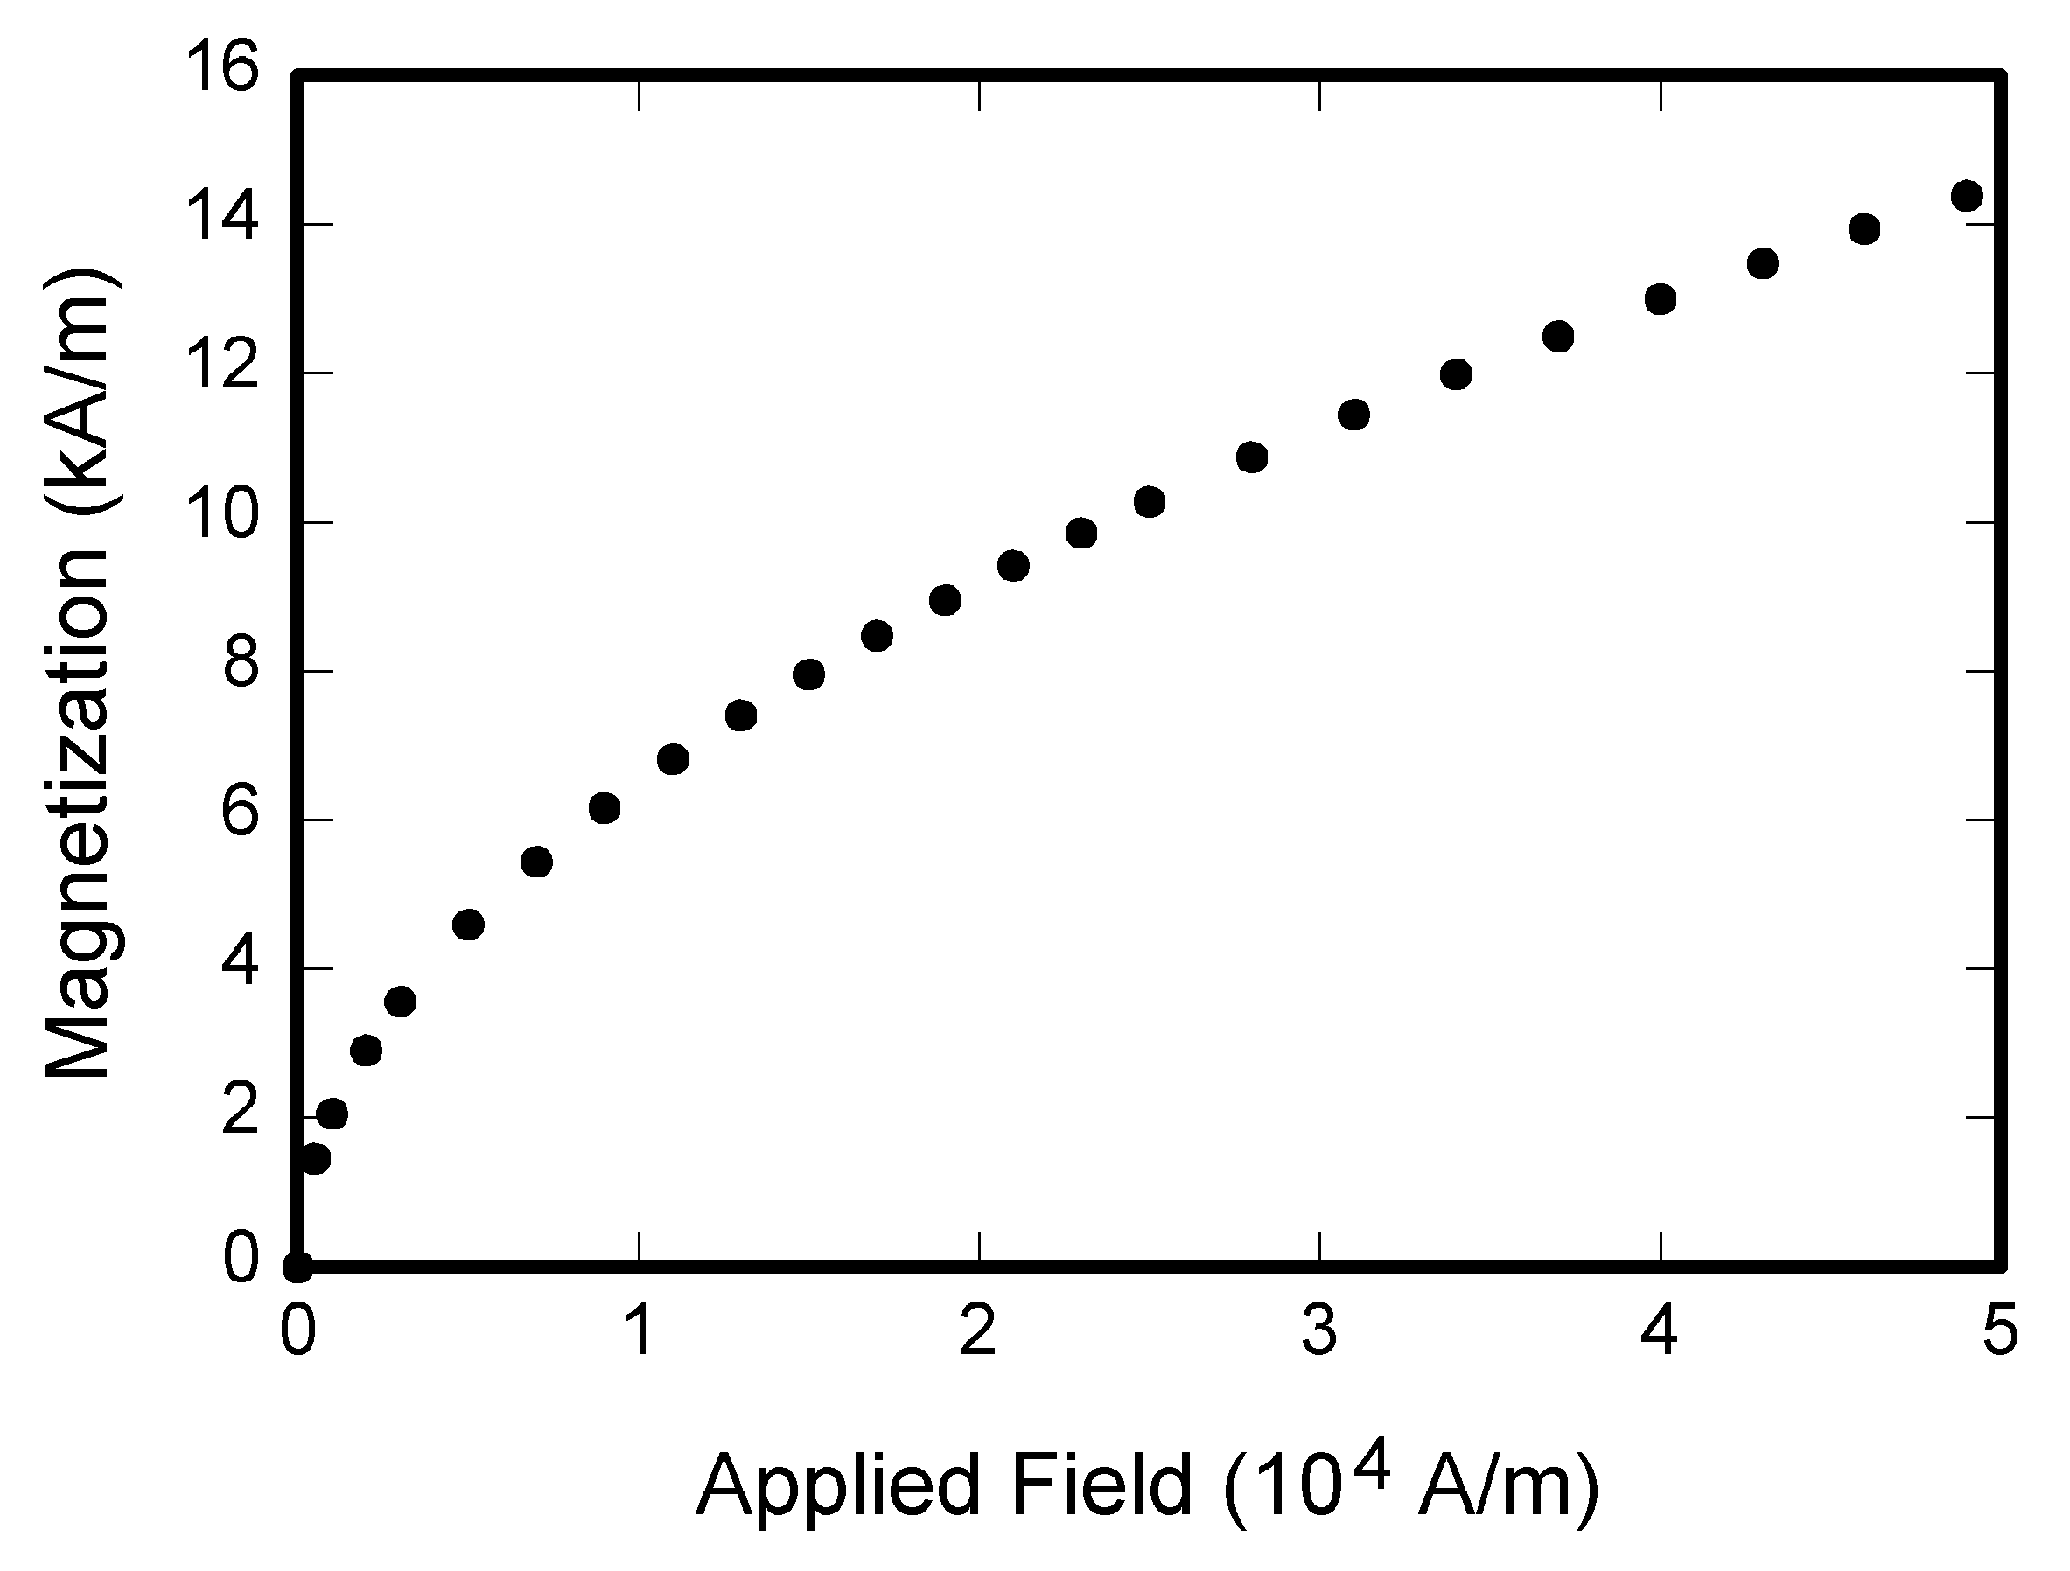
\includegraphics[width=\linewidth]{./fig1.png}
	\caption{Magnetization as a function of applied field. Note that “Fig.” is abbreviated. There is a period after the figure number, followed by two spaces. It is good practice to explain the significance of the figure in the caption.}
	\label{fig:examplesinglefig}
\end{figure}


\begin{table}[ht]
	\begin{center}	
		\small
		\resizebox{1\columnwidth}{!}{
			\begin{tabular}{ m{0.15\columnwidth} >{\raggedleft}m{0.35\columnwidth} m{0.5\columnwidth} }	
				\multicolumn{3}{c}{\textsc{Units for Magnetic Properties}} \\
				\hhline{===}
				{Symbol} & {Quantity} & {Conversion from Gaussian and CGS EMU to SI$^{a}$} \\ 
				\hline
				$\Phi$ & magnetic flux & $1~Mx\rightarrow 10^{-8}~Wb= 10^{-8}~V\cdot~S$\\
				B & magnetic flux density, magnetic induction & $1~G\rightarrow 10^{-4}~T= 10^{-4}~Wb/m^{2}$ \\
				H & magnetic field strength & $1~Oe\rightarrow 10^{3}/(4\pi)~A/m$\\
				m & magnetic moment & $1~erg/G=1~emu\rightarrow10^{-3}~A\cdot~m^{2}=10^{-3}A/m$\\
				M & magnetization & $1~erg/(G\cdot~cm^{3})=1~emu/cm^{3}\rightarrow10^{3}~A/m$ \\
				4$\pi$M & magnetization & $1~G \rightarrow10^{3}/(4\pi)~A/m$\\
				$\sigma$ & specific magnetization & $1~erg/(G\dot~g)=1~emu/g \rightarrow1~A\cdot~m^{2}/kg$ \\
				j & magnetic dipole moment & $1~erg/G=1~emu \rightarrow4\pi\times10^{-10}~Wb\cdot~m$\\
				J & magnetic polarization & $1~erg/(G\cdot cm^{3})=1~emu/cm^{3} \rightarrow4\pi\times10^{-4}~T$\\
				$\chi,\kappa$ & susceptibility & $1 \rightarrow4\pi$\\
				$\chi_{\rho}$ & mass susceptibility & $1~cm^{3}/g\rightarrow4\pi\times10{-3}~m^{3}/kg$ \\
				$\mu$ & permeability & $1\rightarrow4~\pi\times10^{-7}~H/m=4\pi\times10{-7}~Wb/(A\cdot~m)$\\
				$\mu_{\rho}$ & relative permeability & $\mu\rightarrow\mu_{r}$ \\
				w,W & energy density & $1~erg/cm^{3} \rightarrow10^{-1}~J/m^{3}$\\
				N,D & demagnetizing factor & $1 \rightarrow1/(4\pi)$\\
				\hhline{===}
				
			\end{tabular}
		}
	\end{center}
	\caption{Vertical lines are optional in tables. Statements that serve as captions for the entire table do not need footnote letters. \\
		$^{a}$Gaussian units are the same as cg emu for magnetostatics; Mx = maxwell, G = gauss, Oe = oersted; Wb = weber, V = volt, s = second, T = tesla, m = meter, A = ampere, J = joule, kg = kilogram, H = henry.
	}
	\label{Exp}
\end{table}
\normalsize

\subsection{Using Labels Within Figures}	
\subsubsection{Figure Axis labels}
Figure axis labels are often a source of confusion. Use words rather than symbols. As an example, write the quantity "Magnetization," or "Magnetization M," not just "M." Put units in parentheses. Do not label axes only with units. As in Fig. 1, for example, write “Magnetization (A/m)” or “Magnetization (A m$^1$),” not just “A/m.” Do not label axes with a ratio of quantities and units. For example, write “Temperature (K),” not “Temperature/K.” 
Figure labels should be legible, approximately 8 to 10 point type.\\

\subsubsection{Subfigure Labels in Multipart Figures and Tables}
Multipart figures should be combined and labeled before final submission. Labels should appear centered below each subfigure in 8 point Times New Roman font in the format of (a) (b) (c). 

\subsection{Referencing a Figure or Table Within Your Paper}
When referencing your figures and tables within your paper, use the abbreviation “Fig.” even at the beginning of a sentence. Do not abbreviate “Table.” Tables should be numbered with Roman Numerals.

\subsection{Checking Your Figures: The IEEE Graphics Checker}
The IEEE Graphics Checker Tool enables authors to pre-screen their graphics for compliance with IEEE Transactions and Journals standards before submission. The online tool is located at \underline{http://graphicsqc.ieee.org/}. For more information on using the Graphics Checker Tool 
or any other graphics related topic, contact the IEEE Graphics Help Desk by e-mail at \underline{graphics@ieee.org}.
